\documentclass[conference]{IEEEtran}
\IEEEoverridecommandlockouts
% The preceding line is only needed to identify funding in the first footnote. If that is unneeded, please comment it out.
% \usepackage{cite}
\usepackage{amsmath,amssymb,amsfonts}
\usepackage{algorithmic}
\usepackage{graphicx}
\usepackage{textcomp}
\usepackage{xcolor}
\usepackage{tabularray}
\usepackage{cleveref}
\UseTblrLibrary{varwidth}
\usepackage{float}
\usepackage[backend=bibtex,
	bibstyle=numeric,
	citestyle=numeric,
	sorting=nyt,
	url=false,
	maxcitenames=2,
	maxnames=2,
	% dashed=false,
	giveninits=true]{biblatex}
\bibliography{references}
% \def\BibTeX{{\rm B\kern-.05em{\sc i\kern-.025em b}\kern-.08em
%     T\kern-.1667em\lower.7ex\hbox{E}\kern-.125emX}}
\begin{document}

\title{SECURING HOME NETWORK BY UTILIZING FREE AND OPEN SOURCE ENTERPRISE-GRADE NETWORK FIREWALL
HOSTED ON PERSONAL COMPUTER}

\author{\IEEEauthorblockN{Afiq Nazrie Rabbani}
\IEEEauthorblockA{\textit{Faculty of Computing} \\
\textit{University Teknologi Malaysia}\\
81310 Johor, Malaysia \\
nazrie@graduate.utm.my}
\and
\IEEEauthorblockN{Mohd Fo'ad Rohani}
\IEEEauthorblockA{\textit{Faculty of Computing} \\
\textit{University Teknologi Malaysia}\\
81310 Johor, Malaysia \\
foad@utm.my}
}

\maketitle

\begin{abstract}

  As the application of information and communication technology has become exponentially increased
  over the last few years, smart and intelligent devices started to appear in the home environment.
  The development of wireless technologies created great freedoms for and more mobility of users
  with mobile devices. This also increased the use of mobile devices at home, leading to the birth
  of wireless networks in homes. However, the broad adoption of ICT in households created a new
  security risks and threats against private assets of users inside the home network. It is becoming
  more troublesome as most individuals in the home environment are less skilled and capable to
  respond against intruder and hacker attacks. This project intends to develop a network firewall
  with unique system infrastructure by utilizing bare-metal hypervisor to host firewall virtual
  machine and monitoring containers. This approach allows cost reduction because the utilisation of
  single PC as the host of multiple virtual machines. The system is expected to be able to provide
  proper network security infrastructure for home network environment

\end{abstract}

\begin{IEEEkeywords}
network security, firewall, virtualised, monitoring
\end{IEEEkeywords}

\section{Introduction}

Information and communication technology, in the shape of physical and digital assets, are uniquely
new kinds of personal property in this digital age. Home networks, every device connected to it,
including personal computers and smart devices, and even the data stored inside previously mentioned
devices should be treated carefully and protected under an adequate network security measure.
Personal data and even devices access control are two of many private assets that individual might
not want them to be accessed or even tampered by unknown outsiders. Internet Service Provider (ISP)
on most of the time provide their home internet subscriber a basic router with Wi-Fi capability.
However, the supplied router often has limited capabilities for securing the home network. Home
users can always purchase third party router with more features; however, it will still cost them a
fair amount of money.

\section{Problem Background}

The widespread usage of information and communication technology in households introduces another
type of risks and threats towards ICT assets, both physical and digital form. Additionally,
individuals in the home network environment are far less capable and prepared to address
cyberattacks and intruders. Because of that, individuals at home are clueless to some extent as they
may have no idea what is or may happen to their home, home devices, the data stored within the
devices, and more terrifying, their own personal lives as attackers are now able to do physical harm
to individuals inside the home. Moreover, as detailed by Zetter, it is possible for hackers to
perform attack against home or even business automation and security systems through power lines.
Using this conduit, the hackers can, through remote commands, take control of a multitude of
devices, such as lights, electronic locks, heating and air conditioning systems, and security alarm
and cameras. This exploit is possible as the systems operate on Ethernet networks that communicate
over the existing power lines in the home.

This project is aimed to provide proof-of-concept in developing home network security by utilizing
enterprise-grade firewall deployed on virtualised environment on a personal computer (PC). The
firewall is able to be configured according to the use case of the user, with additional advanced
features and controls which can be found in enterprise firewall appliance. The usage of PC in this
project is intended to make the firewall deployment flexible; any PC that fulfil the minimum
requirements should be able to be used as the host of the firewall system.

\section{Literature Review}

This section will discuss several concepts and technologies which will be used in the proposed
system. There will be discussion regarding computer security concepts according to several
standards, followed by explanation of different types of firewalls and virtualization technologies,
brief explanation of Kubernetes system, and concluded with summary of the chapter.

\subsection{Computer Security}

According to \cite{Paulsen_Byers_2019}, the term computer security can be described as a collection
of actions and rules which ensure confidentiality, integrity, and availability of a certain
information system property. This includes the physical hardware, underlying software, embedded
firmware, and data that is transmitted, saved, and processed.

Derived from above definition, there are three key objectives which are the core of computer
security:

\subsubsection{Confidentiality}

The concept of Confidentiality covers the following two corresponding concepts:

\begin{itemize}

  \item Data confidentiality: Assures that private or confidential information is not made
    accessible or shared to unauthorized users.

  \item Privacy: Assures that personals manage or influence the collection and storage of
    information related to them and by whom and to whom that information may be shared.

\end{itemize}

\subsubsection{Integrity}

The concept of Integrity covers the following two corresponding concepts:

\begin{itemize}

  \item Data integrity: Assures that information and programs are communicated through a particular
    and authorized method.

  \item System integrity: Assures that a system serves its purpose in an unimpaired form, free from
    deliberate or unintended unauthorized manipulation of the system.

\end{itemize}

\subsubsection{Availability}

Assures that systems work properly and service is available authorized users.


\subsection{Threats and Attacks}

RFC 4949 defines four types of threat impacts and enumerates the attack types which lead to each
impact:

\subsubsection{Unauthorized disclosure}

RFC 4949 defines unauthorized disclosure as a situation which an individual acquires access to
certain data albeit the individual is not legitimate. There are four threat actions that could lead
to unauthorized disclosure:

\begin{itemize}

  \item Exposure: An unauthorized individual is able to directly access to critical data.

  \item Interception: An unauthorized individual interrupts critical data transmitted between
    legitimate origins and destinations.

  \item Inference: A condition where an unauthorized individual is able to indirectly accesses
    critical data by understanding from the attributes or results of communications.

  \item Intrusion: A condition where an unauthorized individual gains access to critical data by
    evading or beating the security guard of a system.

\end{itemize}

\subsubsection{Deception}

Deception is a condition which can lead in an authorized individual acquiring counterfeit data and
assuming it to be the actual data. There are three threat actions that could lead to deception:

\begin{itemize}

  \item Masquerade: An unauthorized individual acquires access to a system or executes a harmful
    action by disguising as an authorized individual.

  \item Falsification: A condition where an authorized individual is deceived by counterfeit data.

  \item Repudiation: A condition where an individual tricks another by falsely denying obligation
    for a behavior.

\end{itemize}

\subsubsection{Disruption}

A condition can be categorised as a disruption when there is action that interrupts or prevents the
intended functionality of system services and utilities. There are three threat actions that could
lead to disruption:

\begin{itemize}

  \item Incapacitation: Interrupts system operation by incapacitating a component of the system.

  \item Corruption: Adversely mutates system operation by harmfully altering system data or
    functions.

  \item Obstruction: A condition where system operation is being impeded by a threat which result in
    interruption of system services.

\end{itemize}

\subsubsection{Usurpation}

Usurpation is a condition where an unauthorized individual takeover the control system services or
functions. There are two threat actions that could lead to usurpation:

\begin{itemize}

  \item Misappropriation: A condition where an individual presume unauthorized control of physical
    or logical resource of a certain system.

  \item Misuse: A condition which may lead a system component to execute a function or behavior that
    is harmful to the security of the system.

\end{itemize}

\subsection{Existing System Analysis}

To study and analyze the capabilities and shortcomings of currently existing firewall systems, two
devices are chosen to be inspected: one home router device and one enterprise-grade firewall device.
The first device chosen is Kaon AR2140, the router that provided by Maxis for its Maxis Fiber
subscriber. The Kaon AR2140 main features are support for Wi-Fi 6 and EasyMesh certification.

For the enterprise firewall device, Deciso DEC675 is chosen to be compared. The DEC675 is a desktop
security appliance sold by Deciso, the parent company of OPNsense. While it is commercialized, it
utilizes the open-source OPNsense firewall operating system at its core. The only addition is
limited Business Edition license, which includes access to commercial firmware repository and
professional support. Since it uses OPNsense, it offers the same security and networking features
that offered by OPNsense.

\begin{table}[H]
  \caption{COMPARISON OF EXISTING SYSTEMS}
  \label{table:existing_system_comparison}
  \begin{tblr}{hlines,colspec={|X[c]|X[c]|X[c]|X[c]|}}
    Feature & AR2140 & DEC675 & Proposed System \\
    Firewall rule & - & \checkmark & \checkmark \\
    IDS/IPS & - & \checkmark & \checkmark \\
    Custom DNS Blocklist & - & \checkmark & \checkmark \\
    Monitoring Dashboard & - & \checkmark & \checkmark \\
  \end{tblr}
\end{table}

\Cref{table:existing_system_comparison} shows the comparison between Kaon AR2140, Deciso DEC675, and
the proposed system.

\section{System Development Methodology}

Waterfall model is selected as the proposed system will mainly serve its function with minimal
user-facing interface. This is in accordance with the definition of waterfall model where the
product definition is required to be stable among the course of the development. Another reason is
the project involves hardware development or configuration where manufacturing or procurement cost
are involved. In addition, the developed system appliance could be considered as critical system
which requires extensive safety and security analysis of the solution specification and design.

\subsection{Phases of Selected Methodology}

The Waterfall model is a linear and sequential software development process consisting of several
phases. The Waterfall model initiated with Requirement Gathering and Analysis, followed by System
Design, Implementation, Integration and System Testing, and ended with Deployment and Maintenance.

\begin{enumerate}

  \item Requirement Gathering and Analysis: The Waterfall project methodology is started by
    gathering the project requirements and analyse the collected facts. The system services,
    constraints, and objectives are established with the system users. They are then defined in
    detail and serve as a system specification.

  \item System Design: Following the Requirements Gathering and Analysis is the System Design phase.
    This phase defines the required condition to either software or physical hardware systems.  This
    involves identifying the modules or components of the system, their relationships, and how they
    will interact with each other. It determines the entire system architecture in general view.

  \item Implementation: The Implementation phase is where the design is finalised as a set of
    solution or components. This also includes verification that every implemented components
    fulfill its requirements.

  \item Integration and System Testing: In the Integration and System Testing phase, the particular
    solution or components are configured and assembled as one entire system. To guarantee that the
    project requirements have been fulfilled, the project may only proceed to the Deployment and
    Maintenance phase after the proposed system has been thoroughly tested for its functionality.

  \item Deployment and Maintenance: After the previous phases of system development, design,
    implementation, and testing have been done and passed, the proposed system will be deployed to
    be used based on its use cases and requirements. After the proposed system has been successfully
    deployed, the project will move to the Maintenance phase. This phase will involve addressing
    user feedback, fixing defects or issues discovered after deployment, and making necessary
    updates or enhancements.

\end{enumerate}

\subsection{Technology Used}

To achieve the project objectives defined in previous chapter, the following technology will be
used. The usage of the selected technology explained in this section is based on their capacity to
fulfill the required tasks.

\begin{enumerate}

  \item Proxmox VE: Proxmox VE is a type 1 hypervisor which serves as server management platform for
    enterprise virtualization. Proxmox will be used as the base foundation of the proposed system.
    It allows other subsystems such as OPNsense virtual machine and containers for Pi-hole and the
    monitoring stack to be installed in one PC.

  \item OPNsense: OPNsense is an open-source firewall and routing platform based on FreeBSD. A few
    of its features including traffic shaping, forward caching proxy, OpenVPN client and intrusion
    detection system. OPNsense will be used as primary firewall OS of the proposed system. It will
    provide the network-based firewall and network routing for the local network. 

  \item Pi-hole: Pi-hole is a DNS server that has DNS sinkhole feature which protects devices
    connected to the local network from unwanted content, such as advertisement and internet
    tracker, without being required to install any client-side software. Pi-hole will be implemented
    in the proposed system as an advertisement and internet tracker blocker.

  \item Vector: Vector is a data processing pipeline that allows logs and metrics collection,
    transformation, and routing. Vector will be used in the proposed system to filter and sanitise
    syslogs that will be received from other VM and containers. Afterwards, the processed logs will
    be shipped to Loki for log storage.

  \item Grafana Loki: Loki is a log aggregation and storage system which took inspiration from
    Prometheus. Loki allows for efficient indexing of log data as in Loki index is copmrised from
    labels without the original log message. Loki will be used to store the syslog data which is
    forwarded by OPNsense and Pi-hole that consists of firewall action, Suricata IDS, and DNS block
    log.

  \item Prometheus: Prometheus is a system monitoring and alerting toolkit which retrieves and
    stores metrics along with the timestamp at when it was reported and optional labels. Prometheus
    will be used to scrape and store the metrics of OPNsense VM and Pi-hole container. This metric
    will be used by Grafana to create centralised monitoring dashboard.

  \item Grafana: Grafana is an open-source data visualization and monitoring tool used to create
    interactive and customizable dashboards for analyzing and monitoring various data sources.
    Grafana will be used to create centralised monitoring dashboard. This includes VM and container
    system metrics, network access log, firewall action log, and DNS block log. This centralised
    monitoring dashboard allows system administrator monitors the proposed system simpler and
    easier.

\end{enumerate}

\section{Requirement Analysis and Design}

This section will examine the proposed project requirements and system design. Identifying project
requirements and defining the proposed system design are mandatory to successfully deliver the
project objectives and functionalities.

\subsection{Requirement Analysis}

This section will outline the specific features, capabilities, and behavior that the software system
should possess in order to fulfill its intended purpose and meet the needs of its users. The
functional requirements describe what the system should do, rather than how it should be
implemented.

\begin{table}[H]
  \caption{LIST OF FUNCTIONAL REQUIREMENTS}
  \label{table:functional_req}
  \begin{tblr}{hlines,colspec={|l|X[l,m]|}}
    \SetCell[c=1]{c} ID & \SetCell[c=1]{c} Description \\
    FR01 & User shall be able to access another device which exists in the local network \\
    FR02 & User shall be able to access the Internet \\
    FR03 & Administrator shall be able to configure the system using the proposed Ansible code \\
    FR04 & Administrator shall be able to monitor the system metrics and logs \\
  \end{tblr}
\end{table}

\begin{table}[H]
  \caption{LIST OF NON-FUNCTIONAL REQUIREMENTS}
  \label{table:nonfunctional_req}
  \begin{tblr}{hlines,colspec={|l|X[l,m]|}}
    \SetCell[c=1]{c} ID & \SetCell[c=1]{c} Description \\
    NFR01 & The system shall be accessible for 24 hours \\
    NFR02 & The system shall have low error rate \\
    NFR03 & The system shall be accessible only by system Administrator \\
  \end{tblr}
\end{table}

\subsection{Design}

\Cref{fig:project_design} shows the proposed system design infrastructure. The system will utilize
Proxmox VE which act as server management platform as its base. Proxmox VE provides KVM hypervisor,
storage and network virtualization for the system. The Proxmox VE will manage virtualised OPNsense
host and local Kubernetes cluster in parallel. The OPNsense host will provide the main network
firewall and routing capabilities. The Pi-hole will be deployed on an LXC container.

\begin{figure}[H]
  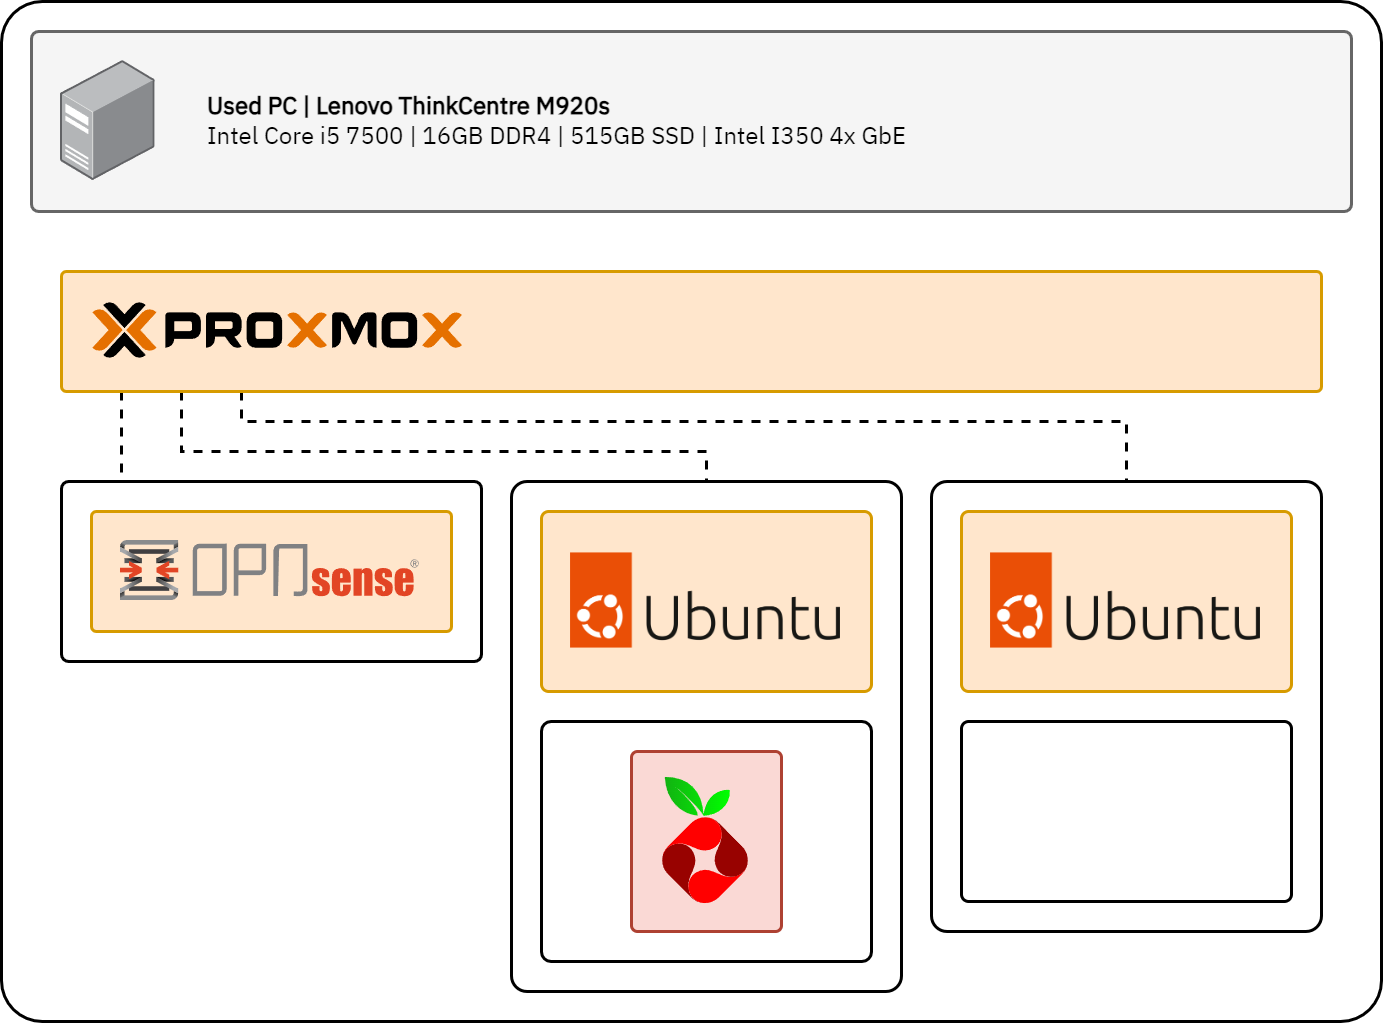
\includegraphics[width=\columnwidth]{../assets/project_design.drawio.png}
  \caption{PROPOSED SYSTEM INFRASTRUCTURE DESIGN}
  \label{fig:project_design}
\end{figure}

\section{Testing}

This section will explain the system implementation which includes the configuration code of the
proposed system that were carried out as continuation from design and analysis stage. This stage is
exceedingly critical for the project to achieve the fulfillment the system requirements. 

Both black-box and white-box testing are utilised to ensure system internals are operating and
behaving correctly to meet the system requirements.

\begin{table}[H]
  \caption{RESULT OF BLACK-BOX TESTING}
  \label{table:black_box}
  \begin{tblr}{hlines,colspec={|l|X[l,m]|c|}}
    \SetCell[c=1]{c} Test Case & \SetCell[c=1]{c} Description & \SetCell[c=1]{c} Result\\
    TC01 & Create opnsense1 VM & PASS \\
    TC02 & Create pihole1 container & PASS \\
    TC03 & Create monitoring1 container & PASS \\
    TC04 & Install Pi-hole using unattended installation & PASS \\
    TC05 & Start Pi-hole service & PASS \\
    TC06 & Install Vector & PASS \\
    TC07 & Configure Vector & PASS \\
    TC08 & Start Vector service & PASS \\
    TC09 & Install Loki & PASS \\
    TC10 & Configure Loki & PASS \\
    TC11 & Start Loki service & PASS \\
    TC12 & Install Prometheus & PASS \\
    TC13 & Configure Prometheus  & PASS\\
    TC14 & Start Prometheus service & PASS \\
    TC15 & Install Grafana & PASS \\
    TC16 & Configure Grafana & PASS \\
    TC17 & Start Grafana service & PASS \\
  \end{tblr}
\end{table}

\begin{table}[H]
  \caption{RESULT OF WHITE-BOX TESTING}
  \label{table:white_box}
  \begin{tblr}{hlines,colspec={|l|X[l,m]|c|}}
    \SetCell[c=1]{c} Test Case & \SetCell[c=1]{c} Description & \SetCell[c=1]{c} Result\\
    TC18 & OPNsense syslog forwarding & PASS \\
    TC19 & OPNsense metric scraping & PASS \\
    TC20 & Pi-hole syslog forwarding & PASS \\
    TC21 & Pi-hole metric scraping & PASS \\
  \end{tblr}
\end{table}

\section{Conclusion}

The proposed system is designed to be an improvement to existing systems. One of the advantages of
this system is the utilization of hypervisor and virtualised environment as the system
infrastructure model. This approach allows multiple guest virtual machines and containers to be
deployed in a single hardware, which is a cost-saving measure for home use.

The only faultless system is a system that is never developed. Based on the outcome of the developed
system, there are several suggestions and improvements that could be applied to enhance the system
on fulfilling the requirements further. Since the beginning of 2023, there are several new mini PC
released that utilise low TDP CPU that could be a good alternative as hardware of this project.
Furthermore, the small dimension of this mini PC allows for easy management and placement. For the
network security suite, there are several options that were identified during the development phases
such as ZenArmor and CrowdSec. These software have its own advantages and disadvantages depending on
the use case. In future improvement, these software could be examined and compared to be used with
this system as an alternative to the current implementation.

\printbibliography[heading=bibintoc]

% \begin{thebibliography}{00}
% \bibitem{b1} G. Eason, B. Noble, and I. N. Sneddon, ``On certain integrals of Lipschitz-Hankel type involving products of Bessel functions,'' Phil. Trans. Roy. Soc. London, vol. A247, pp. 529--551, April 1955.
% \bibitem{b2} J. Clerk Maxwell, A Treatise on Electricity and Magnetism, 3rd ed., vol. 2. Oxford: Clarendon, 1892, pp.68--73.
% \bibitem{b3} I. S. Jacobs and C. P. Bean, ``Fine particles, thin films and exchange anisotropy,'' in Magnetism, vol. III, G. T. Rado and H. Suhl, Eds. New York: Academic, 1963, pp. 271--350.
% \bibitem{b4} K. Elissa, ``Title of paper if known,'' unpublished.
% \bibitem{b5} R. Nicole, ``Title of paper with only first word capitalized,'' J. Name Stand. Abbrev., in press.
% \bibitem{b6} Y. Yorozu, M. Hirano, K. Oka, and Y. Tagawa, ``Electron spectroscopy studies on magneto-optical media and plastic substrate interface,'' IEEE Transl. J. Magn. Japan, vol. 2, pp. 740--741, August 1987 [Digests 9th Annual Conf. Magnetics Japan, p. 301, 1982].
% \bibitem{b7} M. Young, The Technical Writer's Handbook. Mill Valley, CA: University Science, 1989.
% \end{thebibliography}
% \vspace{12pt}
% \color{red}
% IEEE conference templates contain guidance text for composing and formatting conference papers. Please ensure that all template text is removed from your conference paper prior to submission to the conference. Failure to remove the template text from your paper may result in your paper not being published.

\end{document}
